\documentclass[a4paper,12pt]{article}
\usepackage[utf8]{inputenc}
\usepackage[spanish]{babel}
\usepackage{estiloBase}


\title{OpenTSR: \\ Vehículo reconocedor de señales de tráfico}
\author{Alumno: Manuel López Urbina\\Director: Arturo Morgado Estévez}
\date{\today}


\begin{document}

% Este archivo es parte de la memoria del proyecto fin de carrera
% de Manuel López Urbina. Protegida bajo la licencia GFDL.
% Para más información, la licencia completa viene incluida en el
% fichero fdl-1.3.tex
% Fuente tomada del PFC 'libgann' de Francisco Javier Vázquez Púa.
% Fuente tomada de la plantilla LaTeX para
% la realización de Proyectos Final de Carrera de Pablo Recio Quijano.
% Copyright (C) 2008 Francisco Javier Vázquez Púa
% Copyright (C) 2009 Pablo Recio Quijano
% Copyright (C) 2009 Diego Barrios Romero

% Copyright (C) 2012 Manuel López Urbina

\pagestyle{empty}
\begin{titlepage}

  \begin{center}

    
\includegraphics[scale=0.2]{logo_uca.png} \\

    \vspace{2.0cm}

    \LARGE{\textbf{ESCUELA SUPERIOR DE INGENIERÍA}} \\

    \vspace{1.0cm}

    \Large{\textbf{INGENIERÍA TÉCNICA EN INFORMÁTICA DE SISTEMAS}} \\

    \vspace{3.0cm}

    \Large{OpenTSR:\\ Vehículo reconocedor de señales de tráfico} \\

    \vspace{2.0cm}

    \Large{Manuel López Urbina} \\

    \vspace{0.5cm}

    \large{\today}

  \end{center}
\end{titlepage}


\maketitle
\pagestyle{empty}
\abstract{\noindent El siguiente documento se presenta a modo de resumen complementario a la memoria del Proyecto Fin de Carrera de mismo título, entregado el día de la presentación de este proyecto. El proyecto que nos ocupa trata el desarrollo y puesta de funcionamiento de un vehículo robótico dotado de un software reconocedor de las señales de tráfico situadas en su entorno mediante técnicas propias de la visión artificial y del reconocimiento de patrones.}
\tableofcontents 

\cleardoublepage
\pagestyle{plain}
\section{Introducción y antecedentes}

En la actualidad, los robots comerciales e industriales son ampliamente utilizados y realizan tareas de forma más exacta o más barata que los humanos. También se les utiliza en trabajos demasiado sucios, peligrosos o tediosos. Los robots son muy utilizados en plantas de fabricación, montaje y embalaje, en transporte, en exploraciones en la Tierra y en el espacio, cirugía, armamento, investigación en laboratorios y en la producción en masa de bienes industriales o de consumo. Otras aplicaciones incluyen la limpieza de residuos tóxicos, minería, búsqueda y rescate de personas y localización de minas terrestres, en definitiva, la robótica está presente en prácticamente cualquier ámbito de la actualidad.\\

Por otra parte, ninguno de los sistemas robóticos actuales podrían ser funcionales sin un software adecuado para automatización de tareas, siendo esencial una correcta sincronización entre los diferentes elementos hardware y software implicados con la finalidad de garantizar un correcto funcionamiento del conjunto robótico.\\

Centrándonos en lo anterior y aplicándolo en el campo de la automoción, ocasiona que en la actualidad se empleen importantes esfuerzos por parte de grupos investigadores y fabricantes de automóviles para dotar sus vehículos de los elementos necesarios para proporcionar a sus vehículos de un sistema de conducción autónoma. Campo en la actualidad en pleno desarrollo y presentando multitud problemas aún por resolver.\\

Entre los problemas existentes en los sistemas de conducción autónoma destaca su escasa adaptabilidad en carreteras reales donde existen multitud de imperfecciones, como pueden ser el desgaste o la falta de las señales viales, falta de iluminación o existencia de señalización provisional no fija como las indicadoras de obras en la vía. Estas circunstancias especiales impiden el correcto funcionamiento de los vehículos de dentro de unos niveles de seguridad mínimos aceptables para su implantación en carreteras transitables junto con vehículos conducidos de modo tradicional.\\

La problemática actual presentada, junto con que robótica y automoción son mis dos pasiones, hizo que me lanzara a la elaboración de este proyecto que unifica ambos campos anteriormente citados.\\

Así surgió \emph{OpenTSR}.\\

Se trata de un vehículo controlado vía WiFi dotado de una cámara de vídeo la cual visualiza su en torno en busca de aquellas señales de tráfico presentes y actuar en consecuencia.\\

\begin{figure}[H]
  \begin{center}
    
\includegraphics[scale=0.3]{imagenes/lente1.png}
  \end{center}
  \label{fig:logo}
 \caption{Logo OpenTSR \protect\footnotemark.}
\end{figure}

\footnotetext{Logotipo elaborado por Noelia Sales Montes para el proyecto OpenTSR.}

\emph{OpenTSR} (que será el nombre del sistema resultante) será una combinación de un elemento hardware (vehículo entre otros) y software (consola de control) surgido como una aproximación a la solución de los citados problemas.\\


\subsection{Objetivos}

El objetivo principal del proyecto es elaborar un software de detección de señales de tráfico mediante el análisis de las imágenes obtenidas a partir de una cámara. Dicho software irá asociado a un vehículo dotado de una cámara para permitir la visualización del terreno además de ser capaz de reconocer las señales de tráfico mostrando en el ordenador la última señal reconocida. Por otra parte, permitirá al vehículo actuar en consecuencia a la señal detectada. En definitiva se desea dotar al vehículo de un sistema de conducción autónoma a partir de señales de tráfico.\\

El sistema a desarrollar, por tanto, dispondrá de dos modos de funcionamiento, el primero de ellos proporciona una conducción a gusto del usuario, el cual podrá controlar a su antojo el vehículo por el entorno que le rodea mediante un joystick o haciendo uso de las teclas del teclado de un ordenador. En el segundo modo de funcionamiento, el vehículo actuará automáticamente según las señales de tráfico detectadas por la cámara, siendo capaz de ajustar velocidad o realizar giros y paradas de manera automática según los elementos visionados a través de la cámara.

\section{Acerca de este documento}

El documento se ha sido elaborado en un lenguaje sencillo y claro para permitir que un estudiante universitario de cualquier Ingeniería Informática pueda comprender los contenidos sin apenas dificultad añadida.\\

Este documento se organiza en los siguientes capítulos:

\begin{itemize}

\item En el capítulo primero, Introducción, se comentan las razones que han motivado la creación de este proyecto, así como el propósito del mismo.

\item En el capítulo segundo, Conceptos básicos, se incluyen definiciones de aquellos conceptos considerados de interés para la correcta comprensión del contenido de la presente memoria.

\item En el capítulo tercero, Herramientas utilizadas, se realiza una descripción de las diferentes elementos hardware y software empleados durante el desarrollo del proyecto y necesarios para la utilización del mismo.

\item En el capítulo cuarto, Organización temporal, se recoge todo lo que concierne a la distribución y duración de cada una de las tareas llevadas a cabo durante el desarrollo del proyecto que el presente documento describe.

\item En el capítulo quinto, Configuración y montaje de los dispositivos hardware, se explica el proceso seguido para la correcta integración de los dispositivos hardware empleados describiendo la interconexión entre ellos así como su configuración. 

\item En el capítulo sexto, Desarrollo software, se realiza un análisis sobre la metodología empleada para el desarrollo software, describiendo los modelos de ciclo de vida utilizados, la descripción de los requisitos funcionales junto con el diagrama de casos de uso.

\item En el capítulo séptimo, Software de reconocimiento, se hace una descripción explicando los diferentes aspectos y elementos de cada uno de los prototipos desarrollados junto con los problemas encontrados y soluciones adoptadas.

\item En el capítulo octavo, Software de control, se describe cómo se ha llevado a cabo la comunicación ordenador-vehículo a nivel software.

\item En el capítulo noveno, Interfaz gráfica, se recogen aquellos aspectos técnicos de interés referentes a la elaboración de la interfaz gráfica.

\item En el capítulo décimo, Guía de usuario, se describen los diferentes aspectos necesarios para la correcta utilización del conjunto software y hardware de los que se compone el presente proyecto.

\item En el capítulo décimo primero, Conclusiones, se hace mención de las conclusiones obtenidas tras la realización del proyecto además de las posibles mejoras aplicables.

\item En el capítulo Anexos, aparecen los manuales de instalación del software que ha sido necesario para la realización del proyecto.

\end{itemize}


\section{Herramientas utilizadas}

El presente capítulo recoge información acerca de las diferentes herramientas, tanto hardware como software, utilizadas durante el desarrollo del proyecto y para su posterior utilización. 

\subsection {Herramientas software}

El proyecto ha sido realizado haciendo uso del lenguaje de programación C y C++ junto con el uso de diversas bibliotecas. A continuación se realiza una breve descripción de cada una de ellas:

\begin{description} 

\item [OpenCV]
Es una biblioteca libre de visión artificial originalmente desarrollada por Intel. Desde la salida de su primera versión alfa en el mes de enero de 1999, se ha utilizado en infinidad de aplicaciones. Desde sistemas de seguridad con detección de movimiento, hasta aplicaciones para de control de procesos donde es requerido el reconocimiento de objetos. Esto es debido se publica bajo licencia BSD, permitiendo su utilización para propósitos comerciales y de investigación con las condiciones en ella expresadas.

\item [Qt] es una biblioteca multiplataforma ampliamente utilizada para el desarrollo de aplicaciones con una interfaz gráfica de usuario, también es usado para el desarrollo de programas sin interfaz gráfica como herramientas para la línea de comandos y consolas para servidores.

\item [Surveyor Robot Software] software desarrollado por John Cummins junto con los agentes de laboratorio de la Universidad de Brooklyn con la asistencia de M.P. Azhar, y la supervisión del profesor Sklar empleando el lenguaje de programación C++ para el control del vehículo SRV-1 Surveyor. El código está liberado bajo Copyleft.

\item [Simple DirectMedia Layer (SDL)] es un conjunto de bibliotecas desarrolladas en el lenguaje de programación C. Proporciona las funciones básicas para la realización de operaciones de dibujo en dos dimensiones, gestión de efectos de sonido y música, además de carga y gestión de imágenes. Fueron desarrolladas inicialmente por Sam Lantinga, un desarrollador de videojuegos para la plataforma GNU/Linux.

\item [Qt Creator] es un IDE creado por Trolltech para el desarrollo de aplicaciones con las bibliotecas Qt.


\end{description}

\section{Herramientas hardware}
\begin{description}
\item [Vehículo SRV-1]

El elemento hardware principal utilizado es el vehículo \emph{Surveyor SRV-1 WiFi webcam robot}. Dicho vehículo ha sido diseñado para la investigación, la educación, y la exploración, Surveyor SRV-1 es robot que cabe en la palma de la mano, puede desplazarse por superficies lisas y rugosas gracias a sus ruedas tipo tanque fabricadas con caucho. \\

\begin{figure}[H]
  \begin{center}
    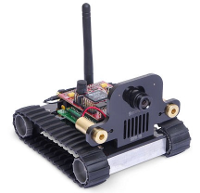
\includegraphics[scale=1]{imagenes/srv-1.png}
  \end{center}
  \caption{Imagen del vehículo SRV-1}
  \label{SRV-1}
\end{figure}

\item [Otros elementos]

Entre el resto de dispositivos hardware se han utilizado:

\begin{itemize}
\item Router
\item Cámara, receptor inalámbrico y capturadora de vídeo
\item Capturadora de vídeo
\item Cámara y receptor inalámbrico
\item Gamepad
\item Ordenador
\end{itemize}

\end{description}

\subsubsection{Licencia}

La aplicación OpenTSR es software libre: usted puede redistribuirlo y / o modificar bajo los términos de la Licencia Pública General de GNU según lo publicado por la Free Software Foundation, ya sea la versión 3 de la Licencia, o (a su elección) cualquier versión posterior.\\

Este programa se distribuye con la esperanza de que sea útil, pero SIN NINGUNA GARANTÍA, incluso sin la garantía implícita de COMERCIALIZACIÓN o IDONEIDAD PARA UN PROPÓSITO PARTICULAR. Ver el GNU General Public License para más detalles.\\

Debería haber recibido una copia de la Licencia Pública General de GNU junto con este programa. Si no es así, consulte \href{http://www.gnu.org/licenses/}{GNU Licenses}.\\

\section{Conceptos básicos}

\subsection{Reconocimiento de patrones}

El reconocimiento de patrones, también llamado lectura de patrones, identificación de figuras y reconocimiento de formas, consiste en el reconocimiento de patrones de señales. Los patrones son obtenidos a partir de procesos de segmentación, extracción de características y descripción para que cada objeto quede representado de manera lo más representativa posible por una colección de descriptores. El sistema de reconocimiento debe asignar a cada objeto su categoría o clase (conjunto de entidades que comparten alguna característica que las hacen diferentes al resto). Para poder reconocer los patrones se siguen tres procesos principales:

\begin{itemize}
 \item Adquisición de datos.
 \item Extracción de características.
 \item Toma de decisiones.
\end{itemize}

La esencia del reconocimiento de patrones es la clasificación, un ejemplo práctico de clasificación puede ser la clasificación de imágenes digitales de letras en las clases de la \emph{A} a la \emph{Z} dependiendo de sus píxeles u otras situaciones que podamos extraer.\\

\begin{figure}[H]
  \begin{center}
    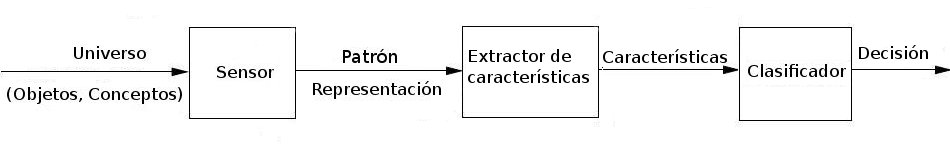
\includegraphics[scale=0.6]{imagenes/Pattern.jpg}
  \end{center}
  \caption{Componentes básicos de un sistema de reconocimiento de patrones.}
  \label{Componentes-basicos-rp}
\end{figure}



\section{Organización temporal}


Para el desarrollo de OpenTSR ha sido necesario emplear varias herramientas, utilidades y bibliotecas. Algunas de ellas, ya habían sido utilizadas en ciertas ocasiones a lo largo de la carrera. Sin embargo, otras han requerido un periodo de formación previo, en el que se han adquirido los conocimientos necesarios para poder desarrollar el proyecto.\\

La mayor parte del proceso de investigación fue dedicado al estudio de las diferentes tecnologías existentes para el procesamiento de imágenes. Se comenzó realizando diferentes prototipos funcionales con Matlab, que además de ser un software privativo, no ofrecía la posibilidad de procesamiento de vídeo en tiempo real debido a su escasa velocidad de cálculo.\\

Posteriormente, tras la necesidad de solventar el problema de la velocidad, se optó por elaborar código con la alternativa libre a Matlab, Octave, implementando las funciones críticas en el lenguaje orientado a objetos C++. Resultando también insuficiente.\\

Continuando con las labores de investigación descubrí una biblioteca de uso muy extendido en robótica llamada OpenCV disponible en C, C++ y Python, resultando la disponible en C especialmente rápida en sus cálculos y proporcionando las características deseadas a las necesidades del proyecto, sobre todo la de dotar al sistema de la capacidad cálculo en tiempo real.\\

Todo ello ha implicado un tiempo bastante considerable en el uso, aprendizaje e investigación de las diferentes tecnologías existentes y comprobar su potencial.\\

Una vez decidida la herramienta para el procesamiento de imágenes, se consideró necesaria la idea de implementar una interfaz acorde con el sistema que permita el visionado de resultados al usuario y el entorno por el que se desplaza el vehículo. Para ello se utilizó la biblioteca Qt escrita en C++. Por tanto fue necesario tiempo para adquirir las nociones básicas de la biblioteca con la ayuda del entorno de desarrollo QtCreator.\\

Por otro lado, existen multitud de algoritmos y técnicas propias del reconocimiento de patrones que no son estudiadas durante la Ingeniería Técnica en Informática y que sí son vistas en la Ingeniería Informática añadiendo la necesidad de estudios de los conceptos propios del reconocimiento de patrones. Todo ello me ha supuesto un esfuerzo de investigación y aprendizaje bastante considerable.\\

Una vez determinadas las diferentes herramientas a utilizar se comenzó con la implementación de los diferentes prototipos funcionales para el software de reconocimiento de imágenes. Finalizado el software de reconocimiento se elaboró el sistema de comunicaciones con el vehículo y la interfaz gráfica.\\

La figura \ref{gantt:tareas} muestra una visión de las diferentes tareas desarrolladas para la elaboración del proyecto junto con la descomposición de cada una de ellas:\\

\begin{figure}[H]
  \begin{center}
    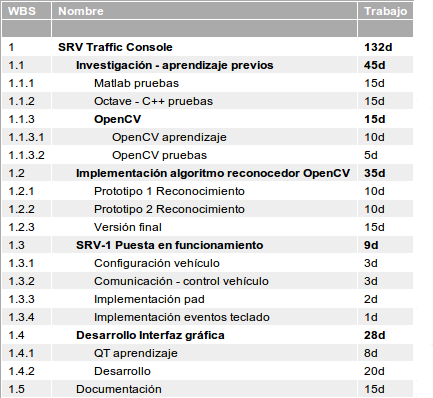
\includegraphics[scale=0.6]{imagenes/tareas-gantt.png}
  \end{center}
  \caption{Descomposición de las tareas implicadas en el desarrollo del proyecto.}
  \label{gantt:tareas}
\end{figure}


\section{Desarrollo software}

\subsection{Metodología de desarrollo}

Este proyecto ha sido obtenido empleando una metodología de desarrollo basada en el modelo de construcción de prototipos para la parte software referente a la visión artificial y una metodología de desarrollo en cascada para el desarrollo de la interfaz gráfica y software de control del vehículo.\\

El modelo de construcción de prototipos proporciona una serie de características que lo hacen idóneo para este proyecto. Dicho modelo resulta especialmente útil en las siguientes situaciones:

\begin{itemize}
\item El cliente define los objetivos generales del software sin entrar en detalles pormenorizados de los requisitos de entrada, procesamiento o salida a obtener.
\item El responsable del desarrollo del software desconoce demasiados aspectos del desarrollo tales como, eficacia de un determinado algoritmo, capacidad de adaptación de un sistema operativo, definición de la interacción hombre-máquina entre otros.
\end{itemize}

Por otro lado, el modelo de desarrollo en cascada resulta adecuado para las siguientes situaciones:

\begin{itemize}
\item Se dispone de unos requisitos claros y precisos.
\item El sistema a desarrollar es de pequeña envergadura.
\item Las tecnologías utilizadas son conocidas por los desarrolladores.
\end{itemize}

Centrándonos nuevamente en el desarrollo del proyecto, los motivos que llevaron a cabo la elección del modelo de desarrollo por prototipos para la obtención del software de visión artificial fueron el amplio desconocimiento existente en cuanto a los algoritmos existentes y su eficacia e idoneidad al producto deseado. \\

En cambio, para el desarrollo de la interfaz gráfica y software de control del vehículo, se optó por el seguimiento del modelo de desarrollo en cascada al tratarse de un desarrollo con una menor dificultad técnica y la disponibilidad de los requisitos necesarios.\\

Por tanto el proyecto queda distribuido en tres subsistemas:

\begin{itemize}
\item Subsistema de visión artificial.
\item Subsistema de control.
\item Subsistema gráfico.
\end{itemize}


\begin{figure}[H]
  \begin{center}
    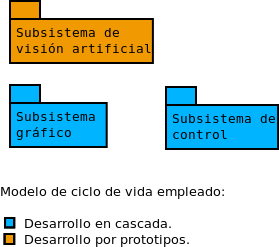
\includegraphics[scale=0.7]{imagenes/subsistemas.png}
  \end{center}
  \caption{Subsistemas existentes en el proyecto junto con el modelo de ciclo de vida utilizado para su desarrollo.}
  \label{subsistemas}
\end{figure}


\section{Software de reconocimiento}

Una vez descritos los diferentes elementos hardware utilizados y la metodología de desarrollo empleada, en el presente capítulo  sucesivos se realizará un profundo análisis de las técnicas y problemas detectados durante el desarrollo, comenzando en el presente tema por el software de reconocimiento. Este subsistema ha sido elaborado siguiendo el modelo de construcción por prototipos.\\

A modo introductorio, destacar que el software de reconocimiento ha sido elaborado haciendo uso de la biblioteca OpenCV para el lenguaje C. Esta biblioteca incluye los elementos necesarios para el tratamiento de imágenes para proporcionar al vehículo de un sistema de reconocimiento de señales de tráfico.\\

Las señales de tráfico detectables por el sistema serán las siguientes:\\

\begin{figure}[H]
  \begin{center}
    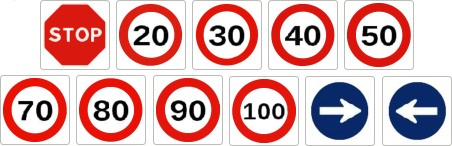
\includegraphics[scale=0.7]{imagenes/seniales2.png}
  \end{center}
  \caption{Conjunto de señales de tráfico detectables por el sistema.}
  \label{conjunto-señales-rp}
\end{figure}

Entre las señales incluidas disponemos las diferentes señales indicadoras de velocidad máxima, existiendo desde la de 20 km/h hasta la de 100 km/h con el objetivo de poder ajustar automáticamente la velocidad del vehículo en función de la señal detectada.\\

Por otro lado existen las señales indicadoras de dirección obligatoria, con el fin de efectuar giros y la señal de stop con el propósito de efectuar paradas de manera automática.\\

Para la elaboración del sistema ha sido necesario el desarrollo de tres prototipos. En el documento del proyecto se describirán cada uno de los ellos junto con los problemas detectados y motivos por los que finalmente se acabaron desechando junto con las soluciones adoptadas.


\section{Software de control}

En presente capítulo contiene información relativa a las herramientas software utilizadas y desarrolladas para la realización de la comunicación con el vehículo ordenando acciones como movimientos, modificación de velocidad, entre otros. Todo ello desde el ordenador por parte del usuario.\\

Cabe recordar que la aplicación consta de dos modos de funcionamiento; un modo automático donde los movimientos son realizados a partir de los elementos visionados por la cámara, y un segundo modo donde el vehículo es manejable por el usuario. En este tema de desarrollan ambos aspectos.\\

Para el control del vehículo se ha utilizado un software denominado \emph{Surveyor Robot Software}, el cual ha sido desarrollado por John Cummins junto con los agentes de laboratorio de la Universidad de Brooklyn con la asistencia de M.P. Azhar, y la supervisión del profesor Sklar empleando el lenguaje de programación C++. El código está liberado bajo Copyleft.\\

El código \emph{Surveyor robot software} ha sido ligeramente modificado para adaptarlo a las necesidades del proyecto, la principal modificación añadida ha sido la de añadir un método para permitir la conexión y desconexión con el vehículo. Permitiendo al usuario desconectar y reconectar a su antojo.

\subsection{Control por parte del usuario}

Lo interesante era proporcionar una serie de mecanismos que permitiera mantener un control del vehículo de una manera cómoda y eficaz para el usuario. Los elementos proporcionados para realizar el control del vehículo son el uso del teclado del ordenador y un gamepad.

\subsubsection{Control desde teclado}

Los movimientos clásicos del vehículo, avance, retroceso y giros, han sido ordenados mediante el uso de las teclas de dirección. Para las capturas de los eventos desde el teclado se han utilizado las herramientas proporcionadas por la biblioteca Qt.\\

Por otro lado, el robot SRV-1, al tratarse de un vehículo tipo tanque, presenta la particularidad de poder controlar las velocidades de movimiento de los motores de un mismo lateral por igual permitiendo la realización de giros. Para permitir realizar ambos tipos de giros se pensó en capturar combinaciones de teclas, de tal modo que si se presiona la tecla ``derecha'', el vehículo realice un giro cerrado y si se presiona la tecla ``arriba'' más ``derecha'', el giro será de mayor amplitud.\\

\subsubsection{Control mediante gamepad}

Para hacer más cómodo, aún si cabe, el manejo del vehículo, se decidió incorporar un mando o gamepad, para ello ha sido necesaria la utilización de la biblioteca SDL con el fin de detectar el dispositivo y capturar los eventos correspondientes no presentando dificultades destacables. 

\subsection{Control automático}

Para dotar al vehículo de un sistema de conducción autónoma se han diseñado una serie de respuestas automáticas ordenadas cuando una determinada señal es detectada.\\

Entre el conjunto de señales de tráfico reconocibles por el sistema disponemos de las indicadoras de velocidad máxima. Estas señales detectables varían desde los 20 hasta los 100 km/h. Cuando una determinada velocidad es detectada, ésta debe ser asignada al vehículo con la finalidad de realizar los movimientos de una manera proporcional a la velocidad indicadora de la señal reconocida. \\

En el momento de la detección de la señal de Stop, se ordena su detención manteniéndose intacto el valor de velocidad que se encuentra en ese momento fijado.\\

Para las señales correspondientes a las indicadoras de dirección obligatoria (flechas), se efectúa un giro de manera automática.\\

Por otro lado, cuando una señal es detectada, la orden automatizada es enviada al vehículo una sola vez de tal modo que si en el entorno apareciese más adelante la misma señal reconocida anteriormente, ésta no se volverá a realizar. Lo que quiere decir que no se reconoce la misma señal de tráfico dos veces seguidas. \\

\section{Interfaz gráfica}

Dada las características del proyecto, era necesario proporcionar a la aplicación de una interfaz gráfica sencilla pero a la vez funcional teniendo como principal objetivo ofrecer al usuario, tras una visión rápida, la localización de los diferentes elementos para control del vehículo y deducir su funcionamiento.\\

En este punto se realiza una descripción de los diferentes elementos presentes en la interfaz gráfica, la cual se compone de dos ventanas, una ventana principal donde se visualiza el estado del vehículo permitiendo su control y una segunda ventana para proporcionar información o ayuda al usuario.\\

Los elementos incorporados en la ventana principal son los siguientes:

\begin{itemize}

\item Panel para el visionado de las imágenes captadas por la cámara.

\item Conjunto de botones para manejo del vehículo, con imágenes representativas de su acción.

\item Panel para el visionado de resultados donde se mostrarán aquellas señales de tráfico detectadas.

\item Información acerca del detector de distancias.

\end{itemize}

La figura \ref{fig:ventana-principal} muestra una imagen de la ventana principal de la aplicación:\\

\begin{figure}[H]
  \begin{center}
    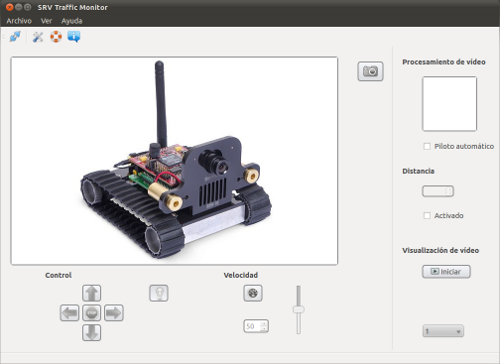
\includegraphics[scale=0.5]{imagenes/ventana-principal.png}
  \end{center}
  \caption{Vista de la ventana principal.}
  \label{fig:ventana-principal}
\end{figure}

En el manual de usuario se encuentra disponible toda la información acerca del modo de utilización de la interfaz gráfica.\\

La ventana secundaria proporcionara información al usuario acerca de los controles del teclado, del gamepad, y otras informaciones de uso como dirección ip del vehículo. Esta ventana ha sido desarrollada con la intención, en mejoras futuras, permitir que dichos parámetros sean configurables.\\

La figura \ref{fig:ventana-información} muestra una imagen de la ventana de información:

\begin{figure}[H]
  \begin{center}
    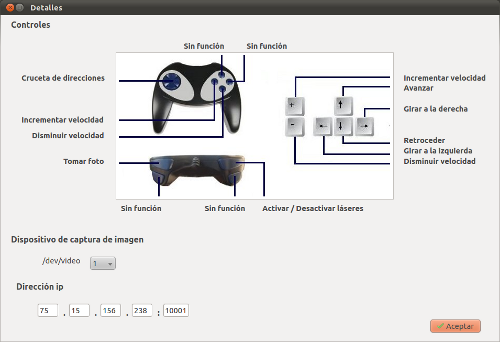
\includegraphics[scale=0.5]{imagenes/ventana-controles.png}
  \end{center}
  \caption{Vista de la ventana de información.}
  \label{fig:ventana-información}
\end{figure}.


\section{Conclusiones}

La elaboración de este proyecto ha resultado muy gratificante a nivel personal. Uno de los motivos principales ha sido la necesidad de trabajar en numerosas áreas de conocimiento entre las que encontramos la programación en los lenguajes C y C++, la robótica y la visión artificial. Algunas de las plataformas mencionadas eran desconocidas al inicio del desarrollo de proyecto y han sido adquiridas tras una amplia labor de investigación y pruebas de desarrollo con diferentes tecnologías como Matlab y Octave sin éxito. Otro de los motivos ha sido la necesidad de continuar con el aprendizaje de conceptos propios de la visión artificial y del reconocimiento de patrones adquiridos mediante la asistencia a asignaturas correspondientes a Ingeniería Informática de segundo ciclo.\\

Entre los elementos desarrollados se destaca:

\begin{itemize}

\item \textbf{Software de procesamiento de imágenes:} escrito en el lenguaje de programación C, utilizando la biblioteca de visión por computador OpenCV. Se han estudiado los principios básicos del procesamiento de imágenes y reconocimiento de patrones aplicados a la visión por computador para construir un sistema software inteligente capaz de controlar un vehículo de manera inalámbrica desplazándose por el entorno actuando según las señales de tráfico existentes. Todo ello en tiempo real.

Ha sido la parte del proyecto en la que más tiempo se ha invertido, el software de reconocimiento de señales de tráfico ha sido obtenido siguiendo una metodología de desarrollo por prototipos habiéndose desarrollado tres prototipos. El algoritmo de clasificación utilizado ha sido el del vecino más cercano. Como datos de entrada se han utilizado las diferentes imágenes de cada uno de los elementos internos de las señales de tráfico dispuestos en columnas y añadidos a la matriz modelos. 

\begin{figure}[H]
  \begin{center}
    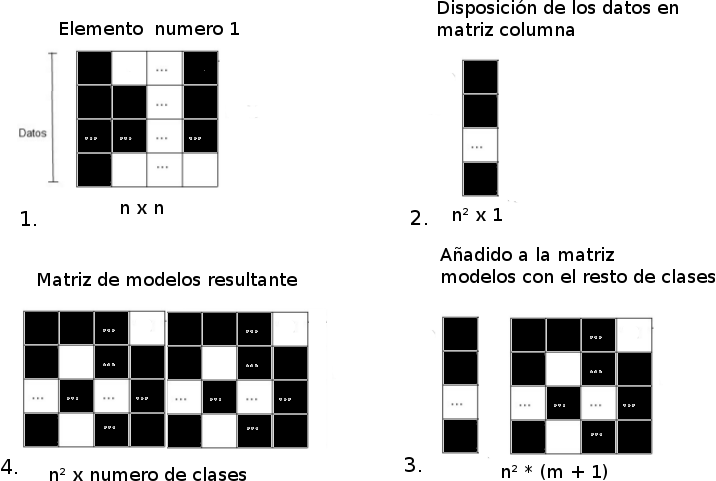
\includegraphics[scale=0.4]{imagenes/entrenamiento.png}
  \end{center}
  \caption{Pasos para la elaboración de la matriz modelos.}
  \label{fig:com-coche-pc}
\end{figure}


Para la clasificación se ha realizado la comparación de la matriz columna obtenida a partir del elemento desconocido con cada una de las columnas existentes en la matriz de modelos. Cada una de ellas corresponde a una clase. La comparación se realiza mediante el cálculo de todas las distancias euclídeas y quedándonos con la clase que menor distancia ha obtenido, es decir, la más cercana o la que guarda más semejanza. Una vez clasificados todos los objetos internos de una señal de tráfico se evalúa el conjunto y se determina la señal de tráfico resultante.  Los elementos internos son analizados siempre que se encuentren dentro de un contorno rojo o azul y sus formas sean las propias de las señales de tráfico, redondas, octogonales,triangulares o cuadradas.


\item \textbf{Software control del vehículo:} se ha empleado el software denominado \emph{Surveyor Robot Software} desarrollado por la universidad de Brooklyn escrito en el lenguaje de programación C++. El software ha sido adaptado a las necesidades del proyecto. Se ha dotado al vehículo de dos modos de funcionamiento, uno de pilotaje tradicional mostrando las señales detectadas por el software de reconocimiento y otro de pilotaje automático realizado a partir de las señales detectadas.

\item \textbf{Interfaz gráfica:} se ha dotado al conjunto de una interfaz gráfica con la finalidad de proporcionar una experiencia de control al usuario mejorada empleando la biblioteca Qt en C++.

\item \textbf{Sistema de comunicaciones:} el proyecto se compone de dos sistemas de comunicaciones, utilizando cada uno de ellos tecnologías distintas:

\begin{itemize}
\item \textbf{Sistema de comunicaciones WiFi:} hace posible el envío de las órdenes desde el ordenador hasta el coche para su control de forma remota. La comunicación se realiza a través de un router donde se conectan ambos dispositivos, el router y el ordenador, formando una infraestructura de red.

\begin{figure}[H]
  \begin{center}
    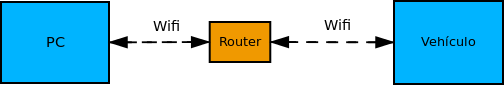
\includegraphics[scale=0.8]{imagenes/comunicacion-coche-robot.png}
  \end{center}
  \caption{Comunicaciones vía WiFi entre el ordenador y el vehículo robótico mediante un router.}
  \label{fig:com-coche-pc}
\end{figure}

\item  \textbf{Sistema de comunicaciones por radiofrecuencia:} hace posible la recepción de imágenes de vídeo desde la cámara al ordenador de forma inalámbrica. Para hacer esto posible se ha dividido el sistema en tres pasos, primeramente se ha comenzando por la recepción inalámbrica de la imagen emitida por la cámara mediante una receptora de imágenes analógicas. A continuación se realiza una conversión de la imagen de vídeo analógica a digital y finalmente se realiza el envío de la imagen digital al ordenador.

\begin{figure}[H]
  \begin{center}
    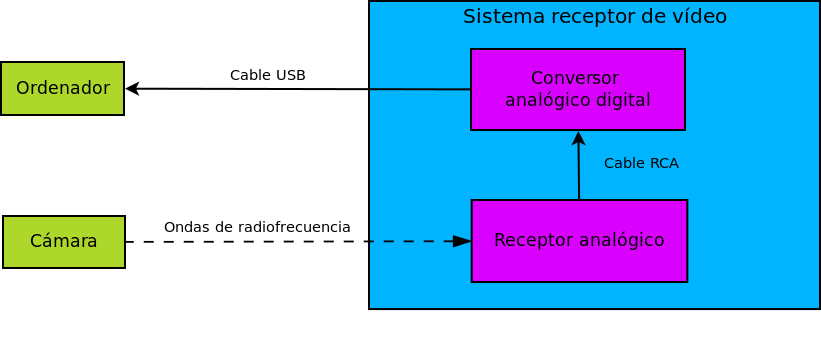
\includegraphics[scale=0.45]{imagenes/esquema-sistema-receptor-video.png}
  \end{center}
  \caption{Elementos implicados en la transmisión de imágenes desde la cámara hasta el ordenador.}
  \label{fig:com-camara-pc}
\end{figure}

\end{itemize}

\end{itemize}

Pienso que el resultado final del proyecto es ideal para aquellas personas aficionadas a la robótica y programación proporcionando una herramienta sea utilizable por la gran comunidad poseedora del vehículo SRV-1 Surveyor en todo el mundo haciéndoles pasar unos momentos divertidos utilizando el vehículo.\\

Una vez presentado podré continuar añadiendo mejoras y muchas cosas que tengo pensadas y que, posiblemente, se realicen para el proyecto de la Ingeniería Informática que me encuentro realizando en la actualidad.

\section{Guía de usuario}

La guía de usuario describirá los objetivos e información de cómo utilizar la aplicación junto con sus diferentes componentes hardware de: OpenTSR.\\

La aplicación OpenTSR ha sido creada por Manuel López Urbina para el proyecto fin de carrera de la titulación de ingeniería técnica informática de la universidad de Cádiz.\\

\subsection{Objetivo de esta guía}

Esta guía tiene como objetivo la de proporcionar al usuario un soporte de ayuda e iniciación a la utilización de los diferentes elementos hardware y software integrantes del proyecto OpenTSR. Esta sección comprende:

\begin{itemize}
\item Guía de acceso a la aplicación.
\item Guía de uso de la aplicación.
\item Guía para la puesta en marcha de los dispositivos hardware.
\item Guía para la configuración de los dispositivos hardware.
\end{itemize}


\clearpage
\nocite{*}
\bibliographystyle{plain}
\bibliography{biblio}
\pagestyle{empty}

\end{document}
